% Options for packages loaded elsewhere
% Options for packages loaded elsewhere
\PassOptionsToPackage{unicode}{hyperref}
\PassOptionsToPackage{hyphens}{url}
\PassOptionsToPackage{dvipsnames,svgnames,x11names}{xcolor}
%
\documentclass[
  letterpaper,
  DIV=11,
  numbers=noendperiod,
  oneside]{scrartcl}
\usepackage{xcolor}
\usepackage[left=1in,marginparwidth=2.0666666666667in,textwidth=4.1333333333333in,marginparsep=0.3in]{geometry}
\usepackage{amsmath,amssymb}
\setcounter{secnumdepth}{-\maxdimen} % remove section numbering
\usepackage{iftex}
\ifPDFTeX
  \usepackage[T1]{fontenc}
  \usepackage[utf8]{inputenc}
  \usepackage{textcomp} % provide euro and other symbols
\else % if luatex or xetex
  \usepackage{unicode-math} % this also loads fontspec
  \defaultfontfeatures{Scale=MatchLowercase}
  \defaultfontfeatures[\rmfamily]{Ligatures=TeX,Scale=1}
\fi
\usepackage{lmodern}
\ifPDFTeX\else
  % xetex/luatex font selection
\fi
% Use upquote if available, for straight quotes in verbatim environments
\IfFileExists{upquote.sty}{\usepackage{upquote}}{}
\IfFileExists{microtype.sty}{% use microtype if available
  \usepackage[]{microtype}
  \UseMicrotypeSet[protrusion]{basicmath} % disable protrusion for tt fonts
}{}
\makeatletter
\@ifundefined{KOMAClassName}{% if non-KOMA class
  \IfFileExists{parskip.sty}{%
    \usepackage{parskip}
  }{% else
    \setlength{\parindent}{0pt}
    \setlength{\parskip}{6pt plus 2pt minus 1pt}}
}{% if KOMA class
  \KOMAoptions{parskip=half}}
\makeatother
% Make \paragraph and \subparagraph free-standing
\makeatletter
\ifx\paragraph\undefined\else
  \let\oldparagraph\paragraph
  \renewcommand{\paragraph}{
    \@ifstar
      \xxxParagraphStar
      \xxxParagraphNoStar
  }
  \newcommand{\xxxParagraphStar}[1]{\oldparagraph*{#1}\mbox{}}
  \newcommand{\xxxParagraphNoStar}[1]{\oldparagraph{#1}\mbox{}}
\fi
\ifx\subparagraph\undefined\else
  \let\oldsubparagraph\subparagraph
  \renewcommand{\subparagraph}{
    \@ifstar
      \xxxSubParagraphStar
      \xxxSubParagraphNoStar
  }
  \newcommand{\xxxSubParagraphStar}[1]{\oldsubparagraph*{#1}\mbox{}}
  \newcommand{\xxxSubParagraphNoStar}[1]{\oldsubparagraph{#1}\mbox{}}
\fi
\makeatother


\usepackage{longtable,booktabs,array}
\usepackage{calc} % for calculating minipage widths
% Correct order of tables after \paragraph or \subparagraph
\usepackage{etoolbox}
\makeatletter
\patchcmd\longtable{\par}{\if@noskipsec\mbox{}\fi\par}{}{}
\makeatother
% Allow footnotes in longtable head/foot
\IfFileExists{footnotehyper.sty}{\usepackage{footnotehyper}}{\usepackage{footnote}}
\makesavenoteenv{longtable}
\usepackage{graphicx}
\makeatletter
\newsavebox\pandoc@box
\newcommand*\pandocbounded[1]{% scales image to fit in text height/width
  \sbox\pandoc@box{#1}%
  \Gscale@div\@tempa{\textheight}{\dimexpr\ht\pandoc@box+\dp\pandoc@box\relax}%
  \Gscale@div\@tempb{\linewidth}{\wd\pandoc@box}%
  \ifdim\@tempb\p@<\@tempa\p@\let\@tempa\@tempb\fi% select the smaller of both
  \ifdim\@tempa\p@<\p@\scalebox{\@tempa}{\usebox\pandoc@box}%
  \else\usebox{\pandoc@box}%
  \fi%
}
% Set default figure placement to htbp
\def\fps@figure{htbp}
\makeatother





\setlength{\emergencystretch}{3em} % prevent overfull lines

\providecommand{\tightlist}{%
  \setlength{\itemsep}{0pt}\setlength{\parskip}{0pt}}



 


% load packages
\usepackage{geometry}
\usepackage{xcolor}
\usepackage{eso-pic}
\usepackage{fancyhdr}
\usepackage{sectsty}
\usepackage{fontspec}
\usepackage{titlesec}

%% Set page size with a wider right margin
\geometry{a4paper, total={170mm,257mm}, left=20mm, top=20mm, bottom=20mm, right=50mm}

%% Let's define some colours
\definecolor{light}{HTML}{E6E6FA}
\definecolor{highlight}{HTML}{800080}
\definecolor{dark}{HTML}{330033}

% %% Let's add the border on the right hand side 
% \AddToShipoutPicture{% 
%     \AtPageLowerLeft{% 
%         \put(\LenToUnit{\dimexpr\paperwidth-3cm},0){% 
%             \color{light}\rule{3cm}{\LenToUnit\paperheight}%
%           }%
%      }%
%      % logo
%     \AtPageLowerLeft{% start the bar at the bottom right of the page
%         \put(\LenToUnit{\dimexpr\paperwidth-2.25cm},27.2cm){% move it to the top right
%             \color{light}\includegraphics[width=1.5cm]{_extensions/nrennie/PrettyPDF/logo.png}
%           }%
%      }%
% }

%% Style the page number
\fancypagestyle{mystyle}{
  \fancyhf{}
  \renewcommand\headrulewidth{0pt}
  \fancyfoot[R]{\thepage}
  \fancyfootoffset{3.5cm}
}
\setlength{\footskip}{20pt}

%% style the chapter/section fonts
\chapterfont{\color{dark}\fontsize{20}{16.8}\selectfont}
\sectionfont{\color{dark}\fontsize{20}{16.8}\selectfont}
\subsectionfont{\color{dark}\fontsize{14}{16.8}\selectfont}
\titleformat{\subsection}
  {\sffamily\Large\bfseries}{\thesection}{1em}{}[{\titlerule[0.8pt]}]
  
% left align title
\makeatletter
\renewcommand{\maketitle}{\bgroup\setlength{\parindent}{0pt}
\begin{flushleft}
  {\sffamily\huge\textbf{\MakeUppercase{\@title}}} \vspace{0.3cm} \newline
  {\Large {\@subtitle}} \newline
  \@author
\end{flushleft}\egroup
}
\makeatother

%% Use some custom fonts
\setsansfont{Ubuntu}[
    Path=_extensions/nrennie/PrettyPDF/Ubuntu/,
    Scale=0.9,
    Extension = .ttf,
    UprightFont=*-Regular,
    BoldFont=*-Bold,
    ItalicFont=*-Italic,
    ]

\setmainfont{Ubuntu}[
    Path=_extensions/nrennie/PrettyPDF/Ubuntu/,
    Scale=0.9,
    Extension = .ttf,
    UprightFont=*-Regular,
    BoldFont=*-Bold,
    ItalicFont=*-Italic,
    ]
\KOMAoption{captions}{tableheading}
\makeatletter
\@ifpackageloaded{caption}{}{\usepackage{caption}}
\AtBeginDocument{%
\ifdefined\contentsname
  \renewcommand*\contentsname{Table of contents}
\else
  \newcommand\contentsname{Table of contents}
\fi
\ifdefined\listfigurename
  \renewcommand*\listfigurename{List of Figures}
\else
  \newcommand\listfigurename{List of Figures}
\fi
\ifdefined\listtablename
  \renewcommand*\listtablename{List of Tables}
\else
  \newcommand\listtablename{List of Tables}
\fi
\ifdefined\figurename
  \renewcommand*\figurename{Figure}
\else
  \newcommand\figurename{Figure}
\fi
\ifdefined\tablename
  \renewcommand*\tablename{Table}
\else
  \newcommand\tablename{Table}
\fi
}
\@ifpackageloaded{float}{}{\usepackage{float}}
\floatstyle{ruled}
\@ifundefined{c@chapter}{\newfloat{codelisting}{h}{lop}}{\newfloat{codelisting}{h}{lop}[chapter]}
\floatname{codelisting}{Listing}
\newcommand*\listoflistings{\listof{codelisting}{List of Listings}}
\makeatother
\makeatletter
\makeatother
\makeatletter
\@ifpackageloaded{caption}{}{\usepackage{caption}}
\@ifpackageloaded{subcaption}{}{\usepackage{subcaption}}
\makeatother
\makeatletter
\@ifpackageloaded{tcolorbox}{}{\usepackage[skins,breakable]{tcolorbox}}
\makeatother
\makeatletter
\@ifundefined{shadecolor}{\definecolor{shadecolor}{rgb}{.97, .97, .97}}{}
\makeatother
\makeatletter
\@ifundefined{codebgcolor}{\definecolor{codebgcolor}{named}{light}}{}
\makeatother
\makeatletter
\ifdefined\Shaded\renewenvironment{Shaded}{\begin{tcolorbox}[colback={codebgcolor}, frame hidden, enhanced, sharp corners, boxrule=0pt, breakable]}{\end{tcolorbox}}\fi
\makeatother
\makeatletter
\@ifpackageloaded{sidenotes}{}{\usepackage{sidenotes}}
\@ifpackageloaded{marginnote}{}{\usepackage{marginnote}}
\makeatother
\usepackage{bookmark}
\IfFileExists{xurl.sty}{\usepackage{xurl}}{} % add URL line breaks if available
\urlstyle{same}
\hypersetup{
  pdftitle={Animated Subjects},
  colorlinks=true,
  linkcolor={highlight},
  filecolor={Maroon},
  citecolor={Blue},
  urlcolor={highlight},
  pdfcreator={LaTeX via pandoc}}


\title{Animated Subjects}
\usepackage{etoolbox}
\makeatletter
\providecommand{\subtitle}[1]{% add subtitle to \maketitle
  \apptocmd{\@title}{\par {\large #1 \par}}{}{}
}
\makeatother
\subtitle{Communicative Fluidity and Social Media Forms}
\author{}
\date{}
\begin{document}
\maketitle

\pagestyle{mystyle}


\marginnote{\begin{footnotesize}

\href{https://www.sunsunlim.com/}{Sun Sun Lim},
``\href{https://journals.sagepub.com/doi/epub/10.1177/2056305115578137}{On
Stickers and Communicative Fluidity in Social Media}''Sunny Yoon,
``\href{https://journals.sagepub.com/doi/epub/10.1177/20563051241292577}{Webtoons,
Desperately Seeking Viewers: Interactive Creativity in Social Media
Platforms and Cultural Appropriation of Global Media Production}''Kate
M. Miltner and Tim Highfield,
``\href{https://journals.sagepub.com/doi/epub/10.1177/2056305117725223}{Never
Gonna GIF You Up: Analyzing the Cultural Significance of the Animated
GIF}''Luke Stark and Kate Crawford,
``\href{https://journals.sagepub.com/doi/epub/10.1177/2056305115604853}{The
Conservatism of Emoji: Work, Affect, and Communication}''

\end{footnotesize}}

\pandocbounded{
\includegraphics[keepaspectratio]{img/kakao-friends.png}}

So far in the course we've talked a lot about
\textbf{content}---influencers, platforms, cultures---but we haven't
talked about \textbf{forms}. So I wanted us to spend a week thinking
about and discussing social media forms that in some cases have become
so familiar and taken for granted that they have become almost
transparent.

Looking at social media forms also opens up the question of cultural
difference, as Sun Sun Lim's short article about stickers reveals.
Animated stickers are a staple of Asian social media and have been the
subject of extensive scholarship for that reason, yet they are less
heavily used in Western and Anglo-American social media culture. It's
interesting to think about why that is, but the reasons are clearly
complex and related to larger cultural differences in societies where
social and cultural norms are clearly very different from those of North
American and European societies. This ``communicative fluidity'', as she
suggests, is related to the concept of ``high-context cultures'' that
she also discusses, and the different social norms around emotional
expression in everyday interacations in particular. In this sense the
widespread use of animated stickers on platforms such as Kakao Talk
(South Korea), WeChat (China), or Line (Japan) can be seen as a kind of
compensatory practice, where they serve to add an emotional register to
plain text messages. We Westerners are all very familiar with using
emoji and animated gifs for this, but the cartoonish nature of animated
stickers not only add a dynamic element to text messages but also an
affective dimension (pronounced \textbf{A}-fect, as in emotion).

An additional aspect of the animated sticker phenonemon in Asian social
media, which Sun Sun Lim doesn't mention, is also maybe so obvious that
it's easily overlooked: that the animations depict \textbf{characters}.
The ubiquity of such communicative characters has been extensively
discussed in academic studies of Asian social media cultures but is
itself part of the larger phenomenon that myself and some other scholars
described as the \textbf{character industry} in the early 2000s (I have
to get around to re-posting the papers from that panel this summer).

Perhaps the best-known recent example of this in the West is the case of
the \href{https://en.wikipedia.org/wiki/Kakao_Friends}{Kakao Friends} in
South Korea:

\url{https://www.youtube.com/embed/fedo9642blU}

These characters started out as sticker mascots and merchandise for the
Kakao Talk mobile chat app, but they have since developed well beyond
that into a major cultural brand that takes a multiplicity of forms
across both digital and material culture, from printed stickers to
plushies to stationery to animated short videos. You can find out more
about them
\href{https://www.knowingkorea.org/contents/view/246/Kakao-Friends-Stores-the-newest-famous-store-in-Hongdae}{here}.
If you have the Kakao Talk app you can even install them in it yourself
from the iPHone
\href{https://apps.apple.com/us/app/hello-kakao-friends/id1451176667}{App
Store}.

The point to keep in mind here is that as ubiquitous as they are, when
it comes to social media characters the Kakao Friends are no more than
the tip of the iceberg. Even on the Kakao Talk platform alone, there are
innumerable animated \textbf{sticker packs} depicting a host of other
animated characters. You can customize these to any aspect of your own
identity, personal style, or sense of humor. Some examples.

\marginnote{\begin{footnotesize}

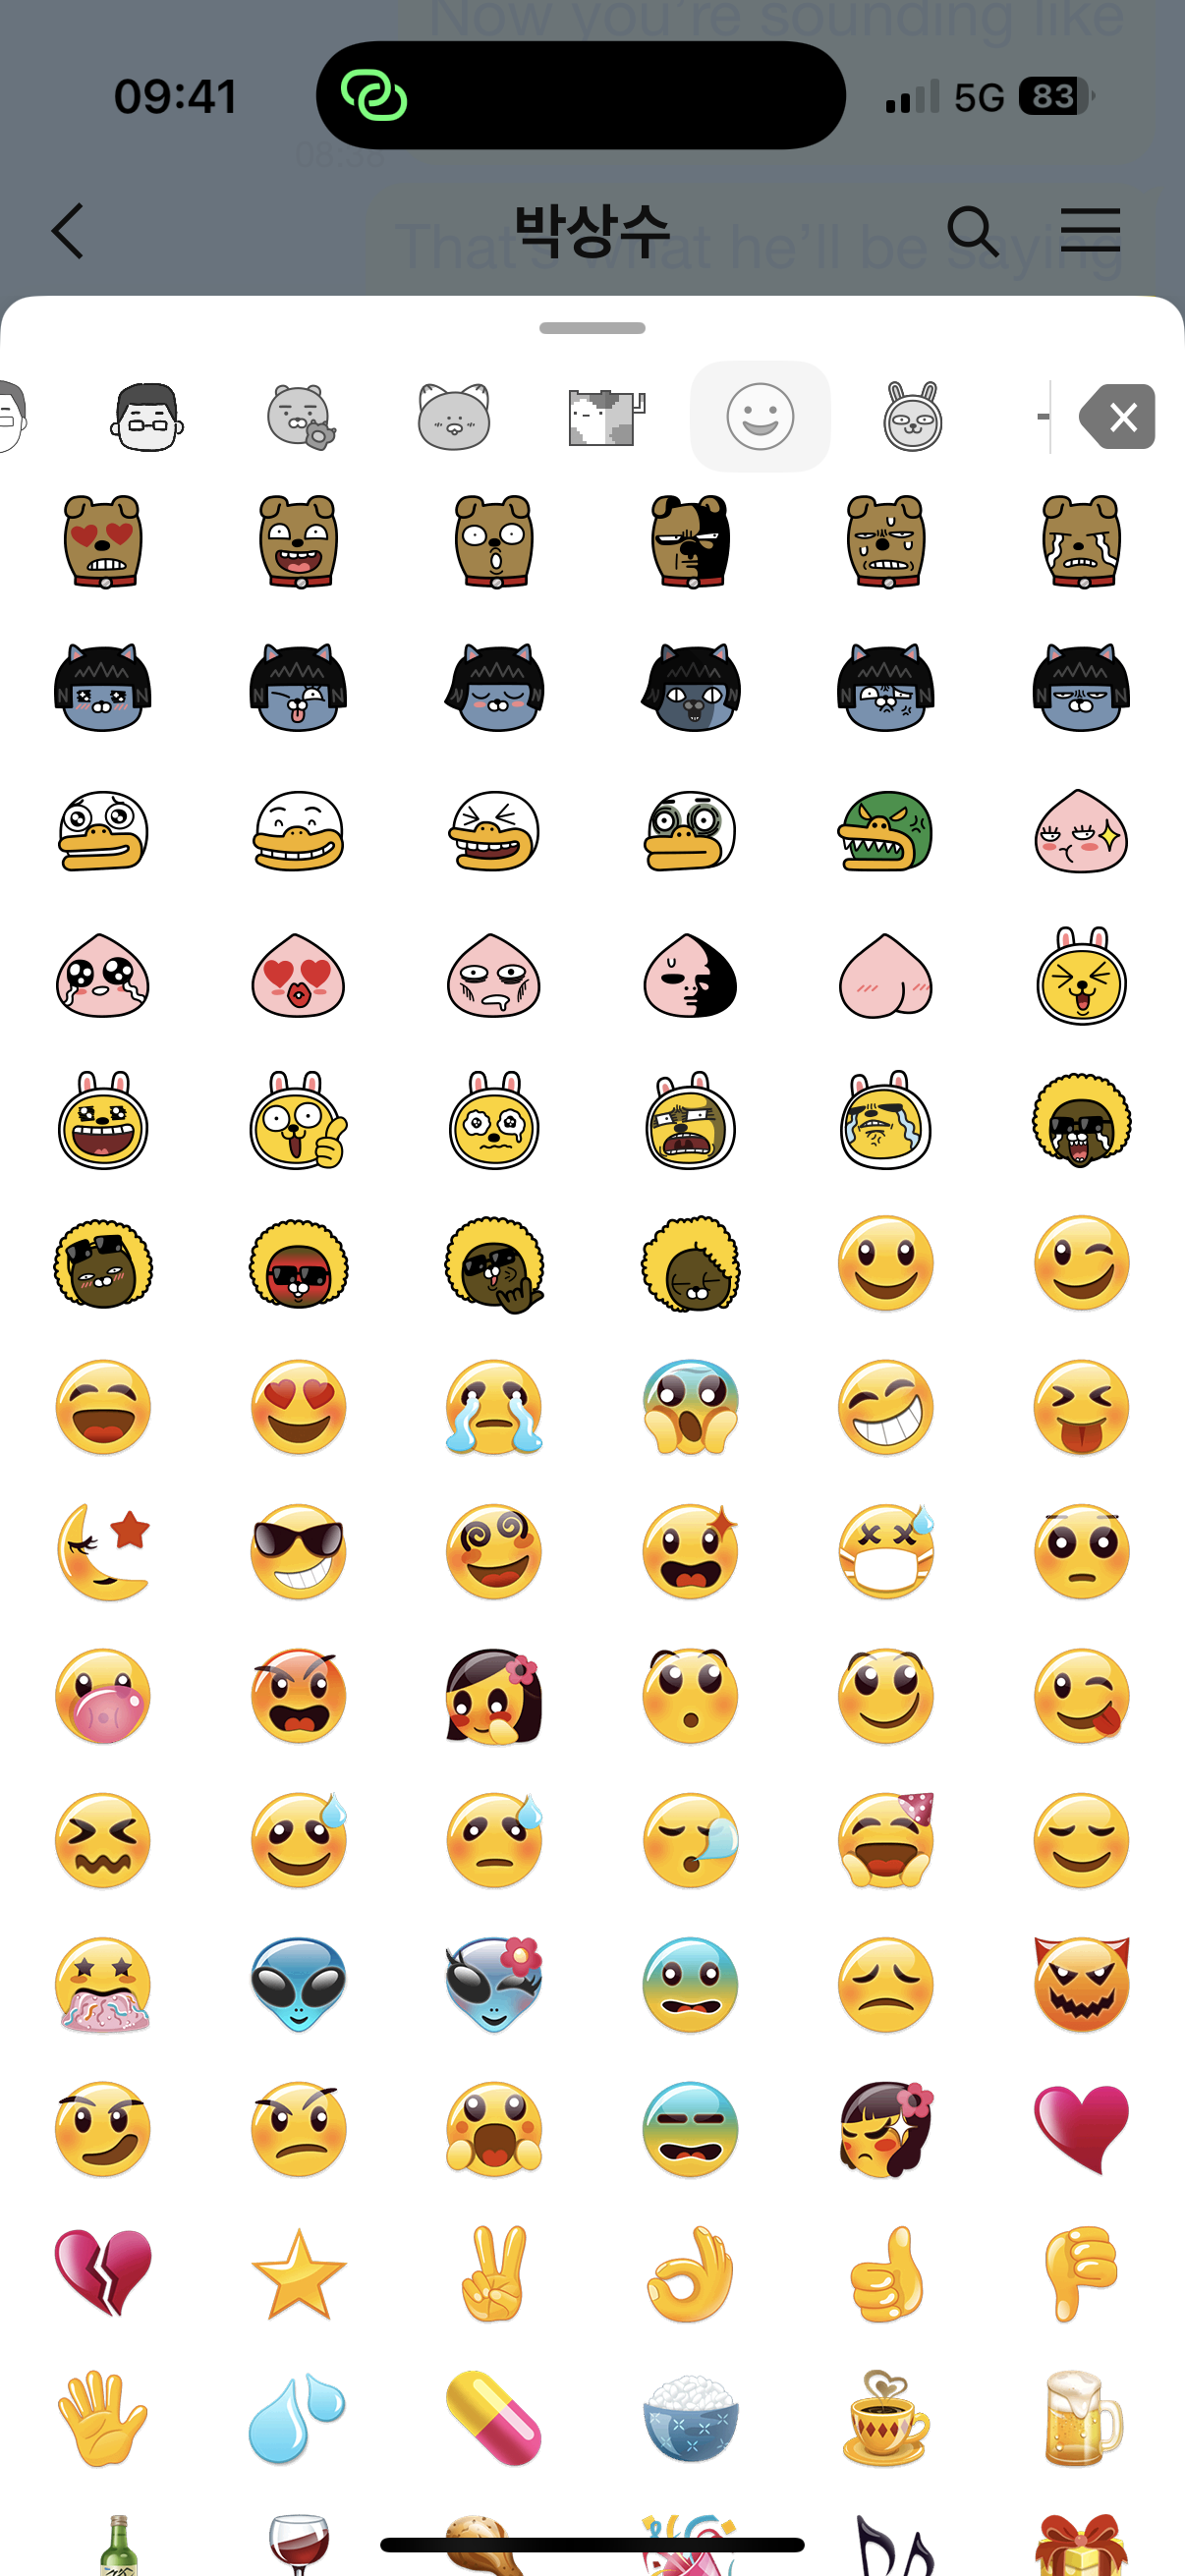
\includegraphics[width=1.04167in,height=\textheight,keepaspectratio]{img/kakao-classic.png}

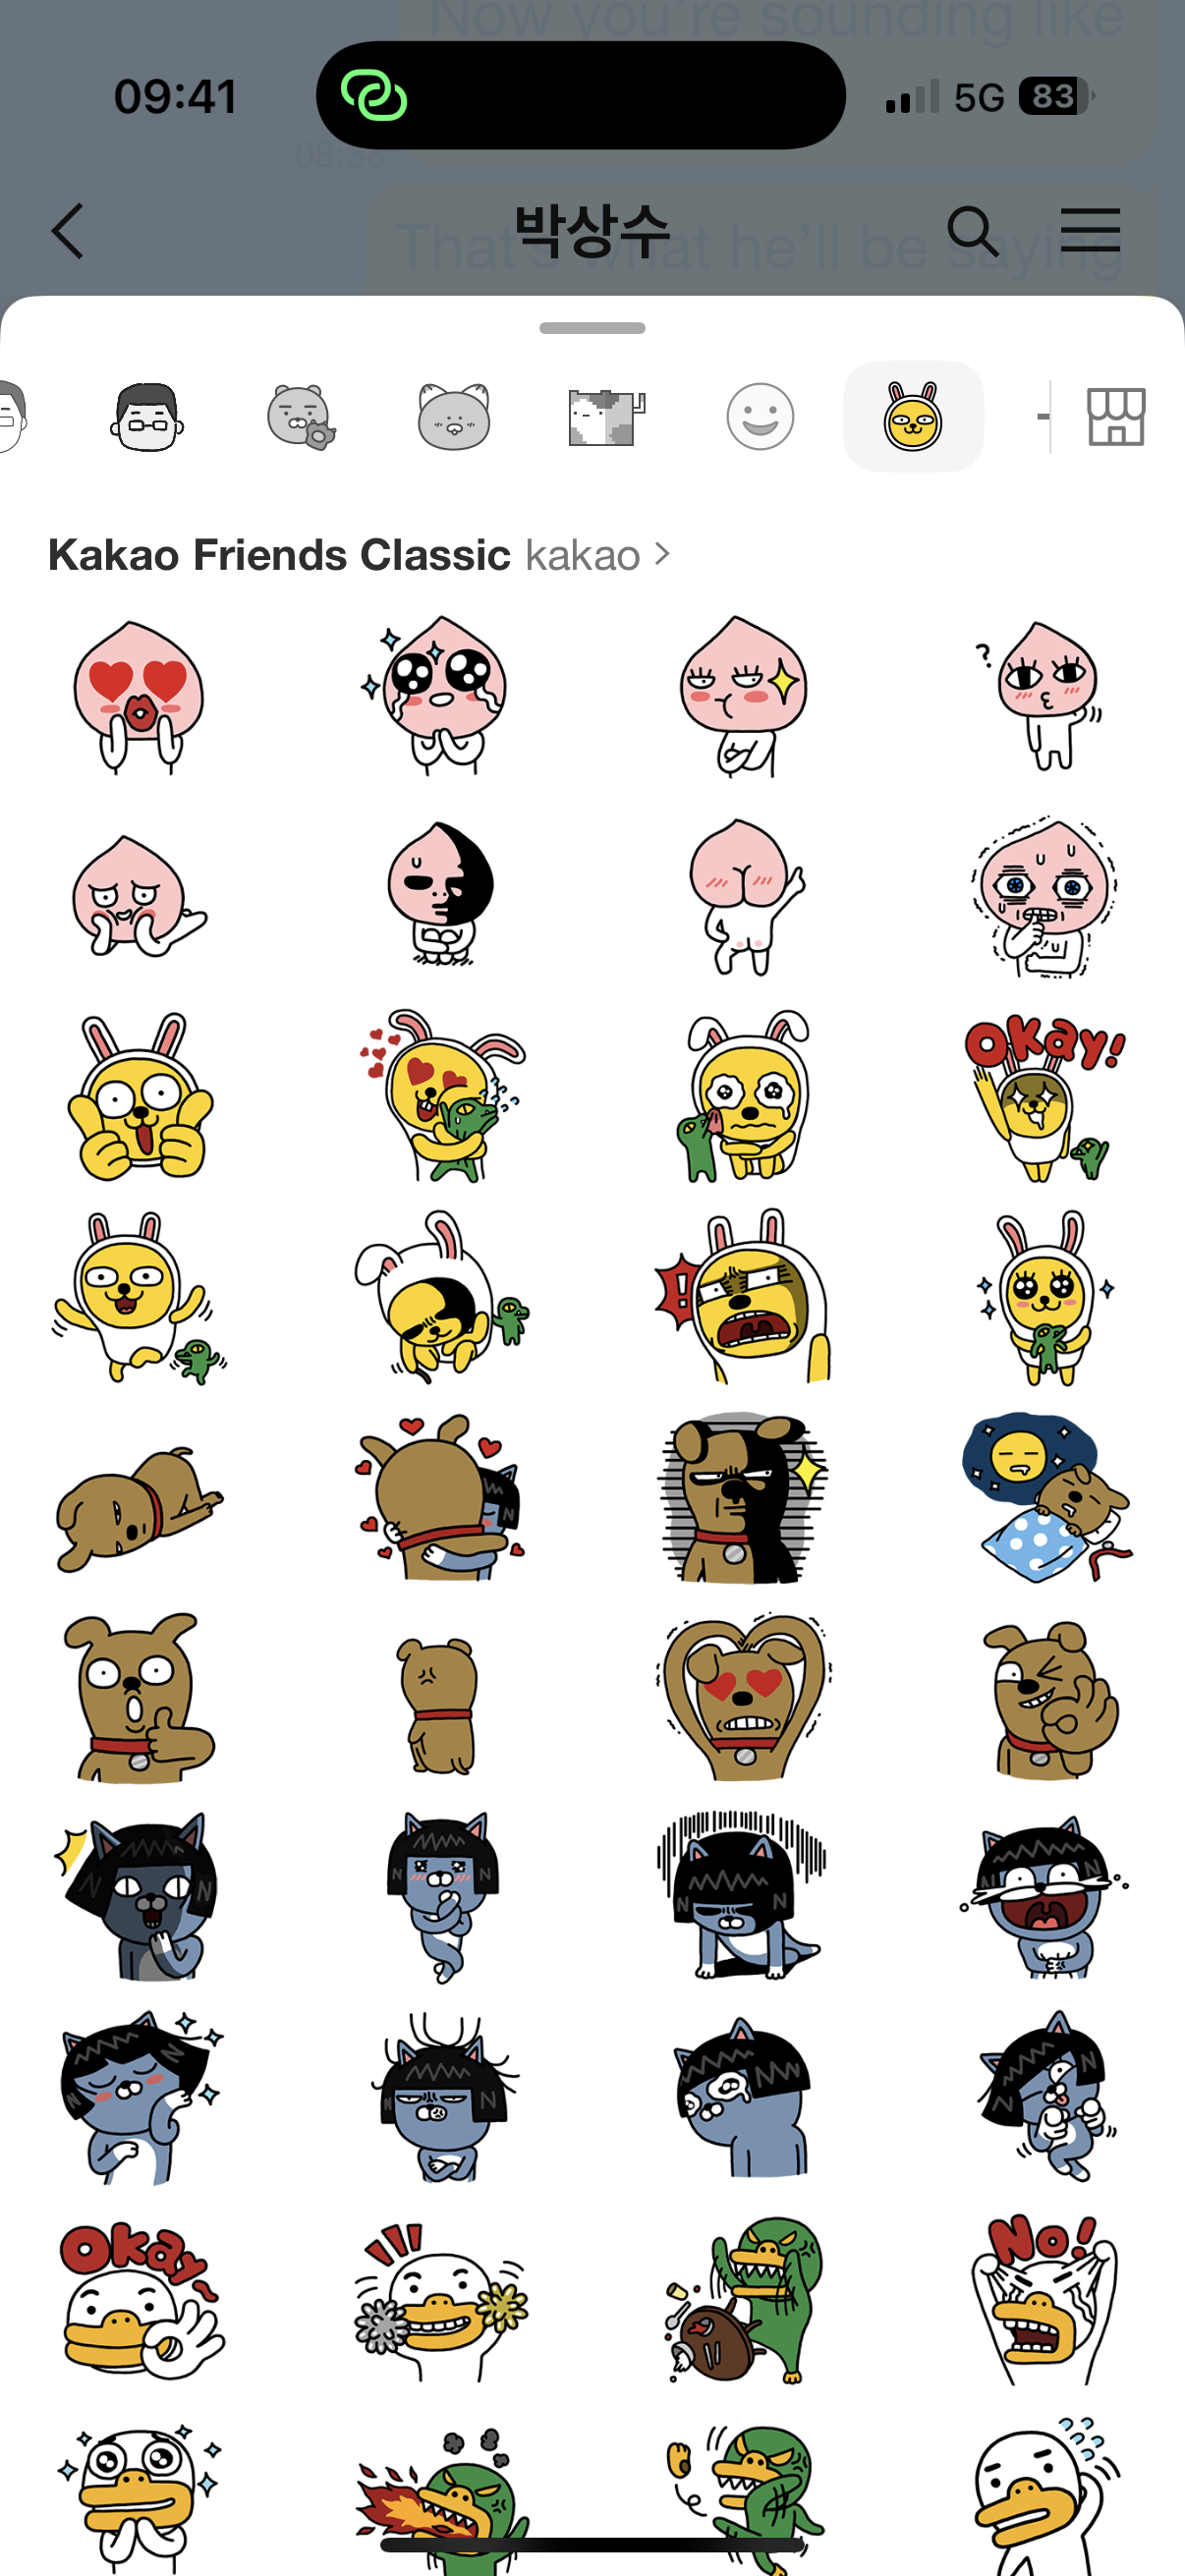
\includegraphics[width=1.04167in,height=\textheight,keepaspectratio]{img/kakaoclassic2.png}

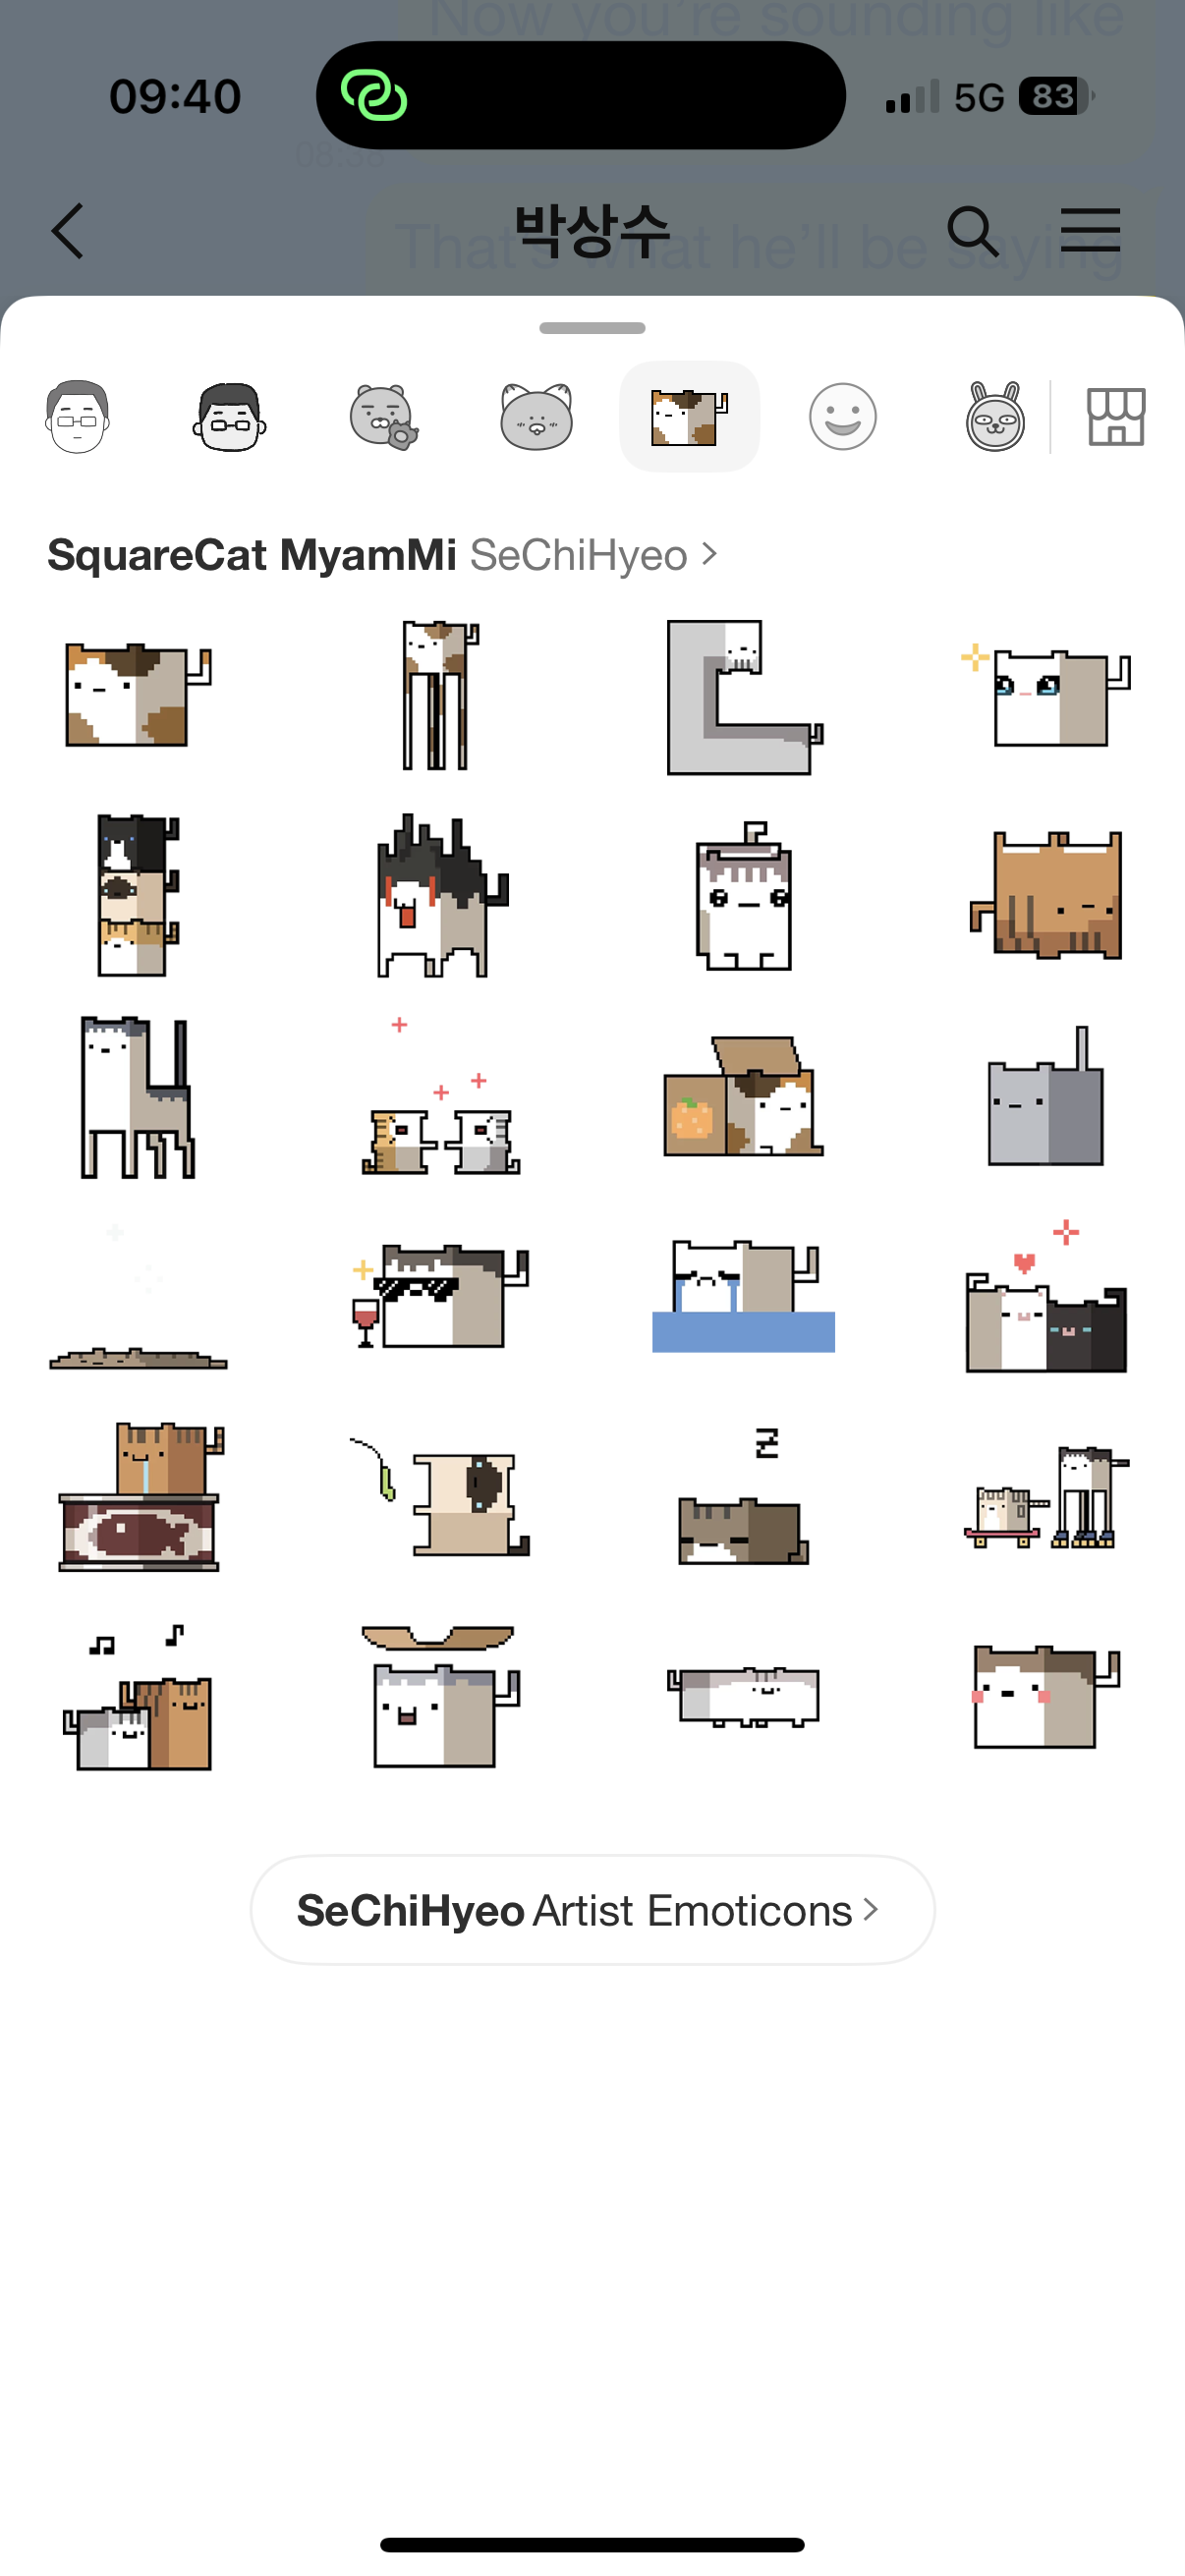
\includegraphics[width=1.04167in,height=\textheight,keepaspectratio]{img/squarecat.png}

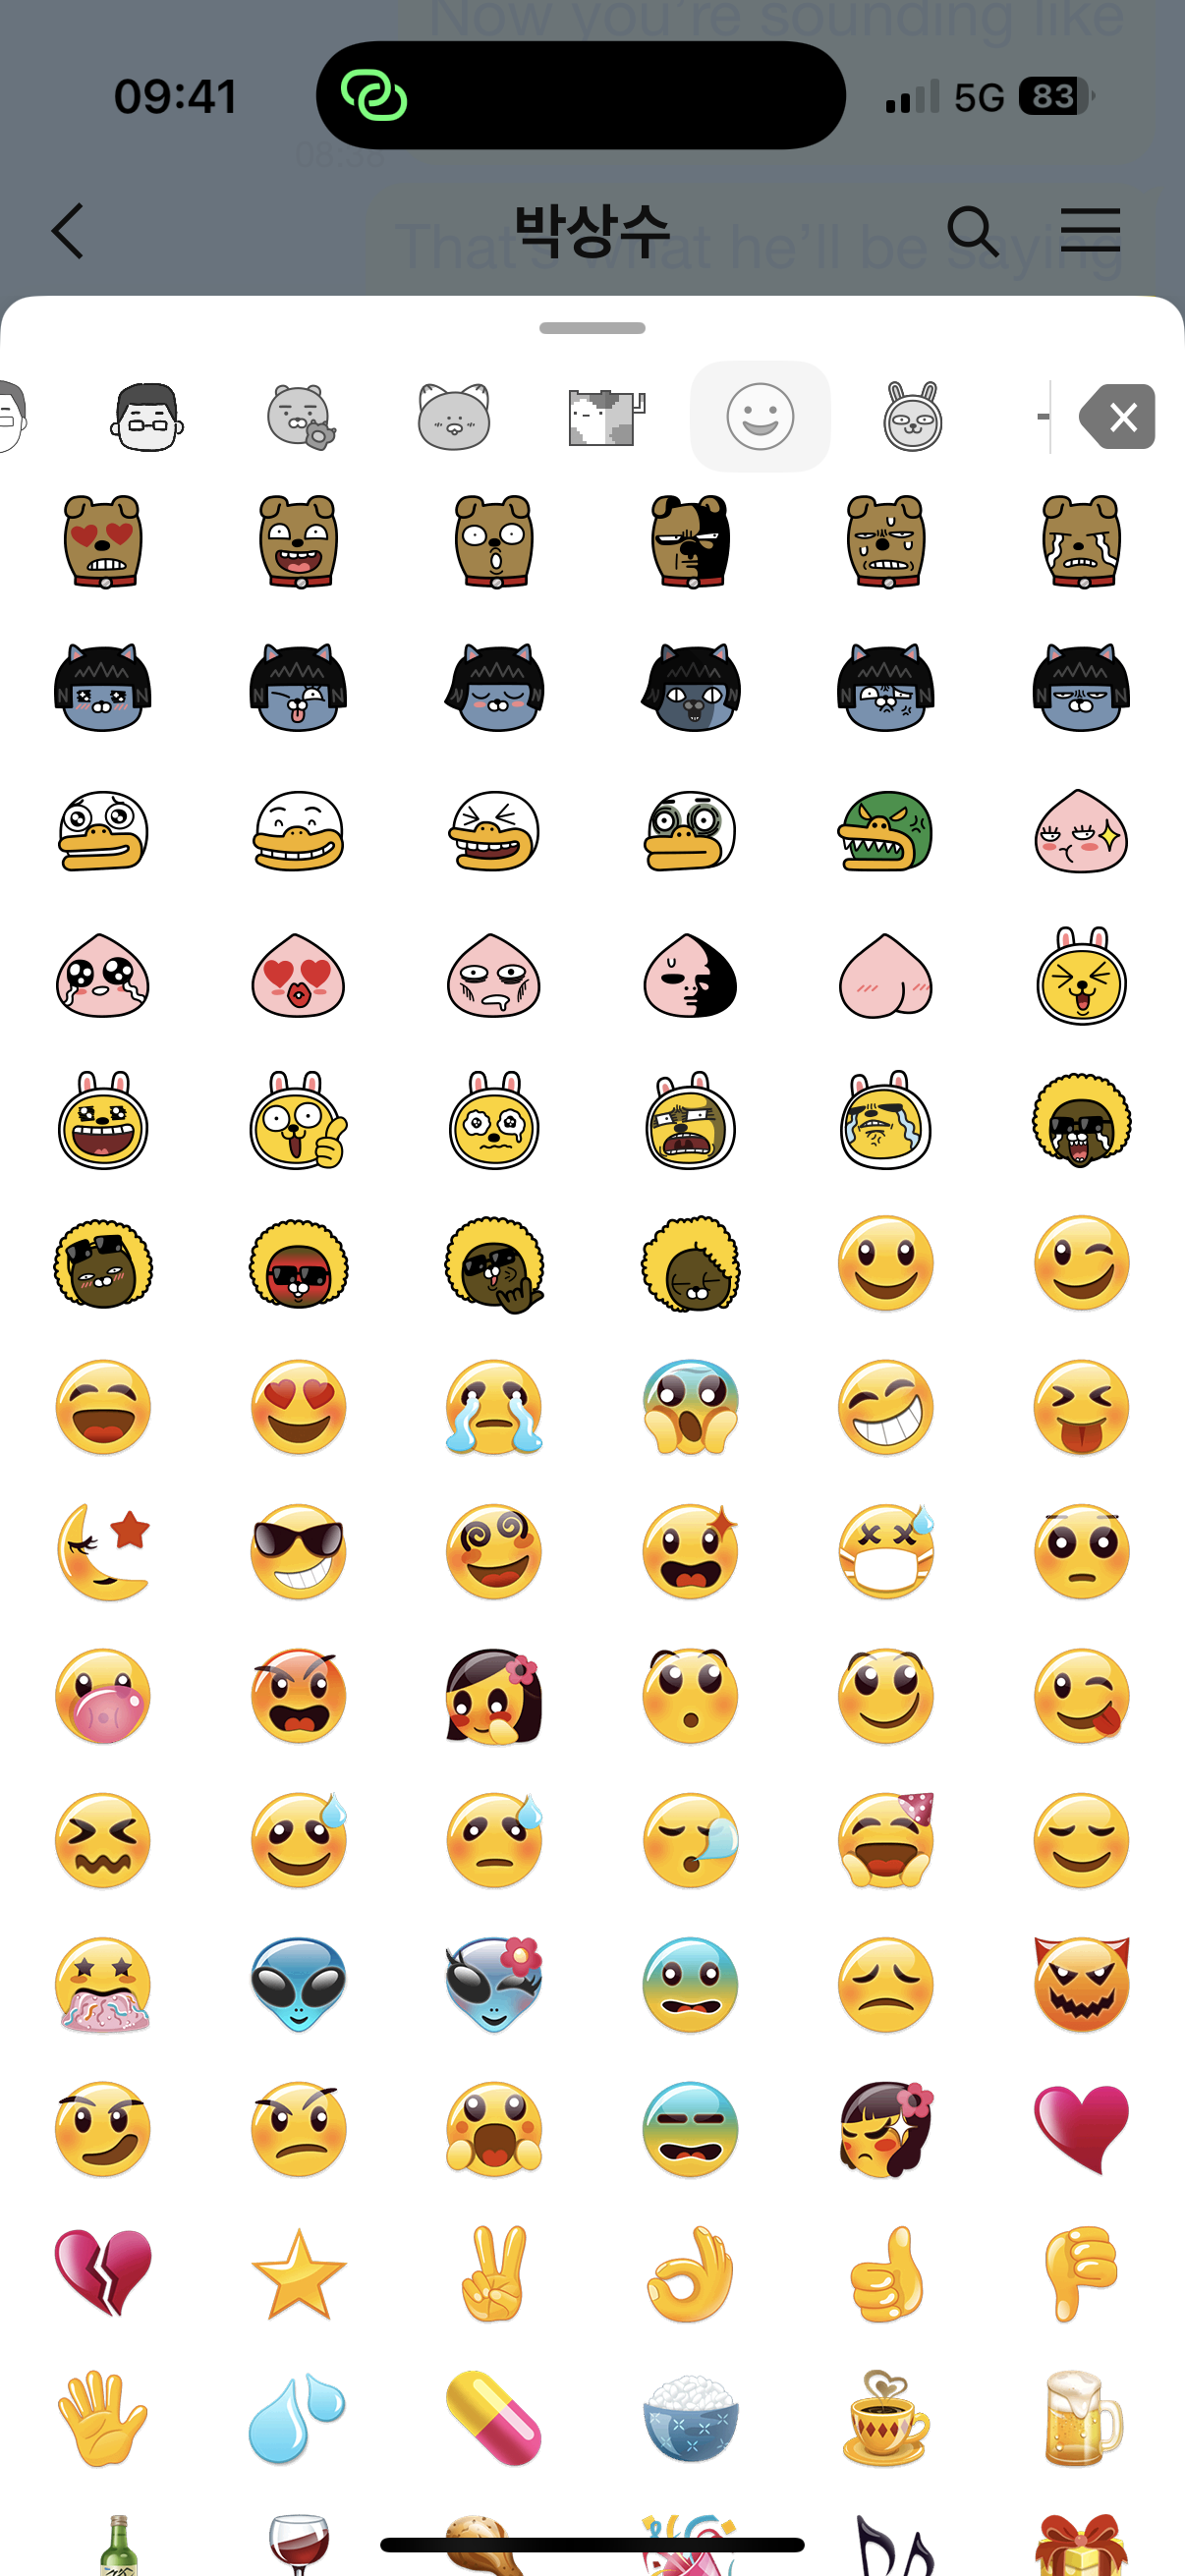
\includegraphics[width=1.04167in,height=\textheight,keepaspectratio]{img/kakao-classic.png}

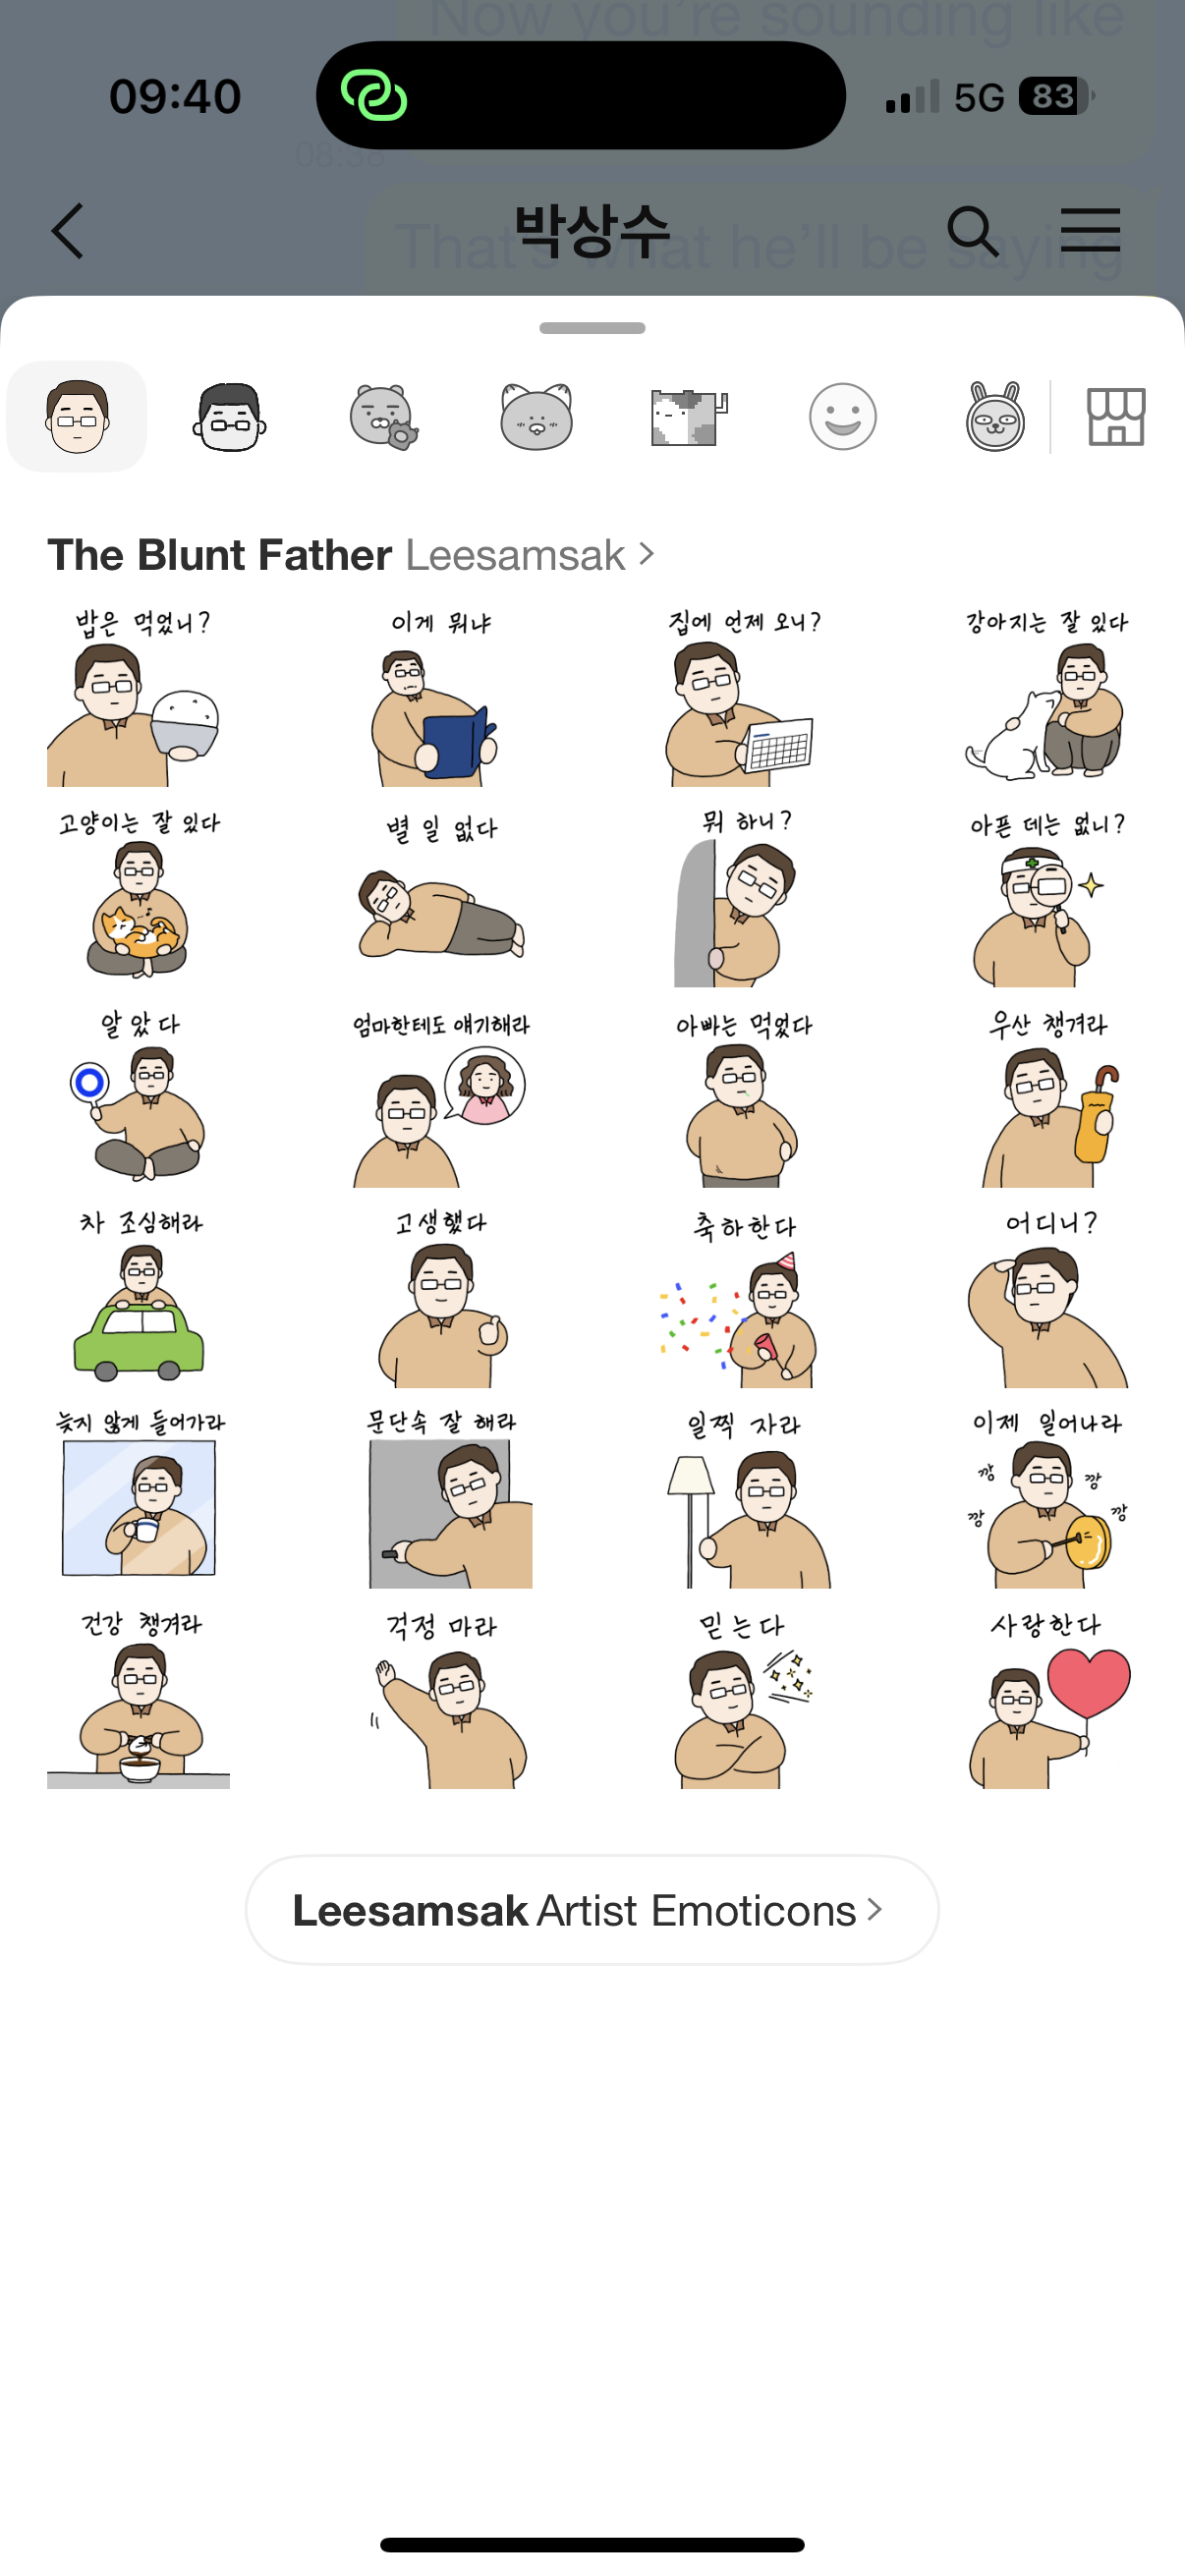
\includegraphics[width=1.04167in,height=\textheight,keepaspectratio]{img/bluntfather1.png}

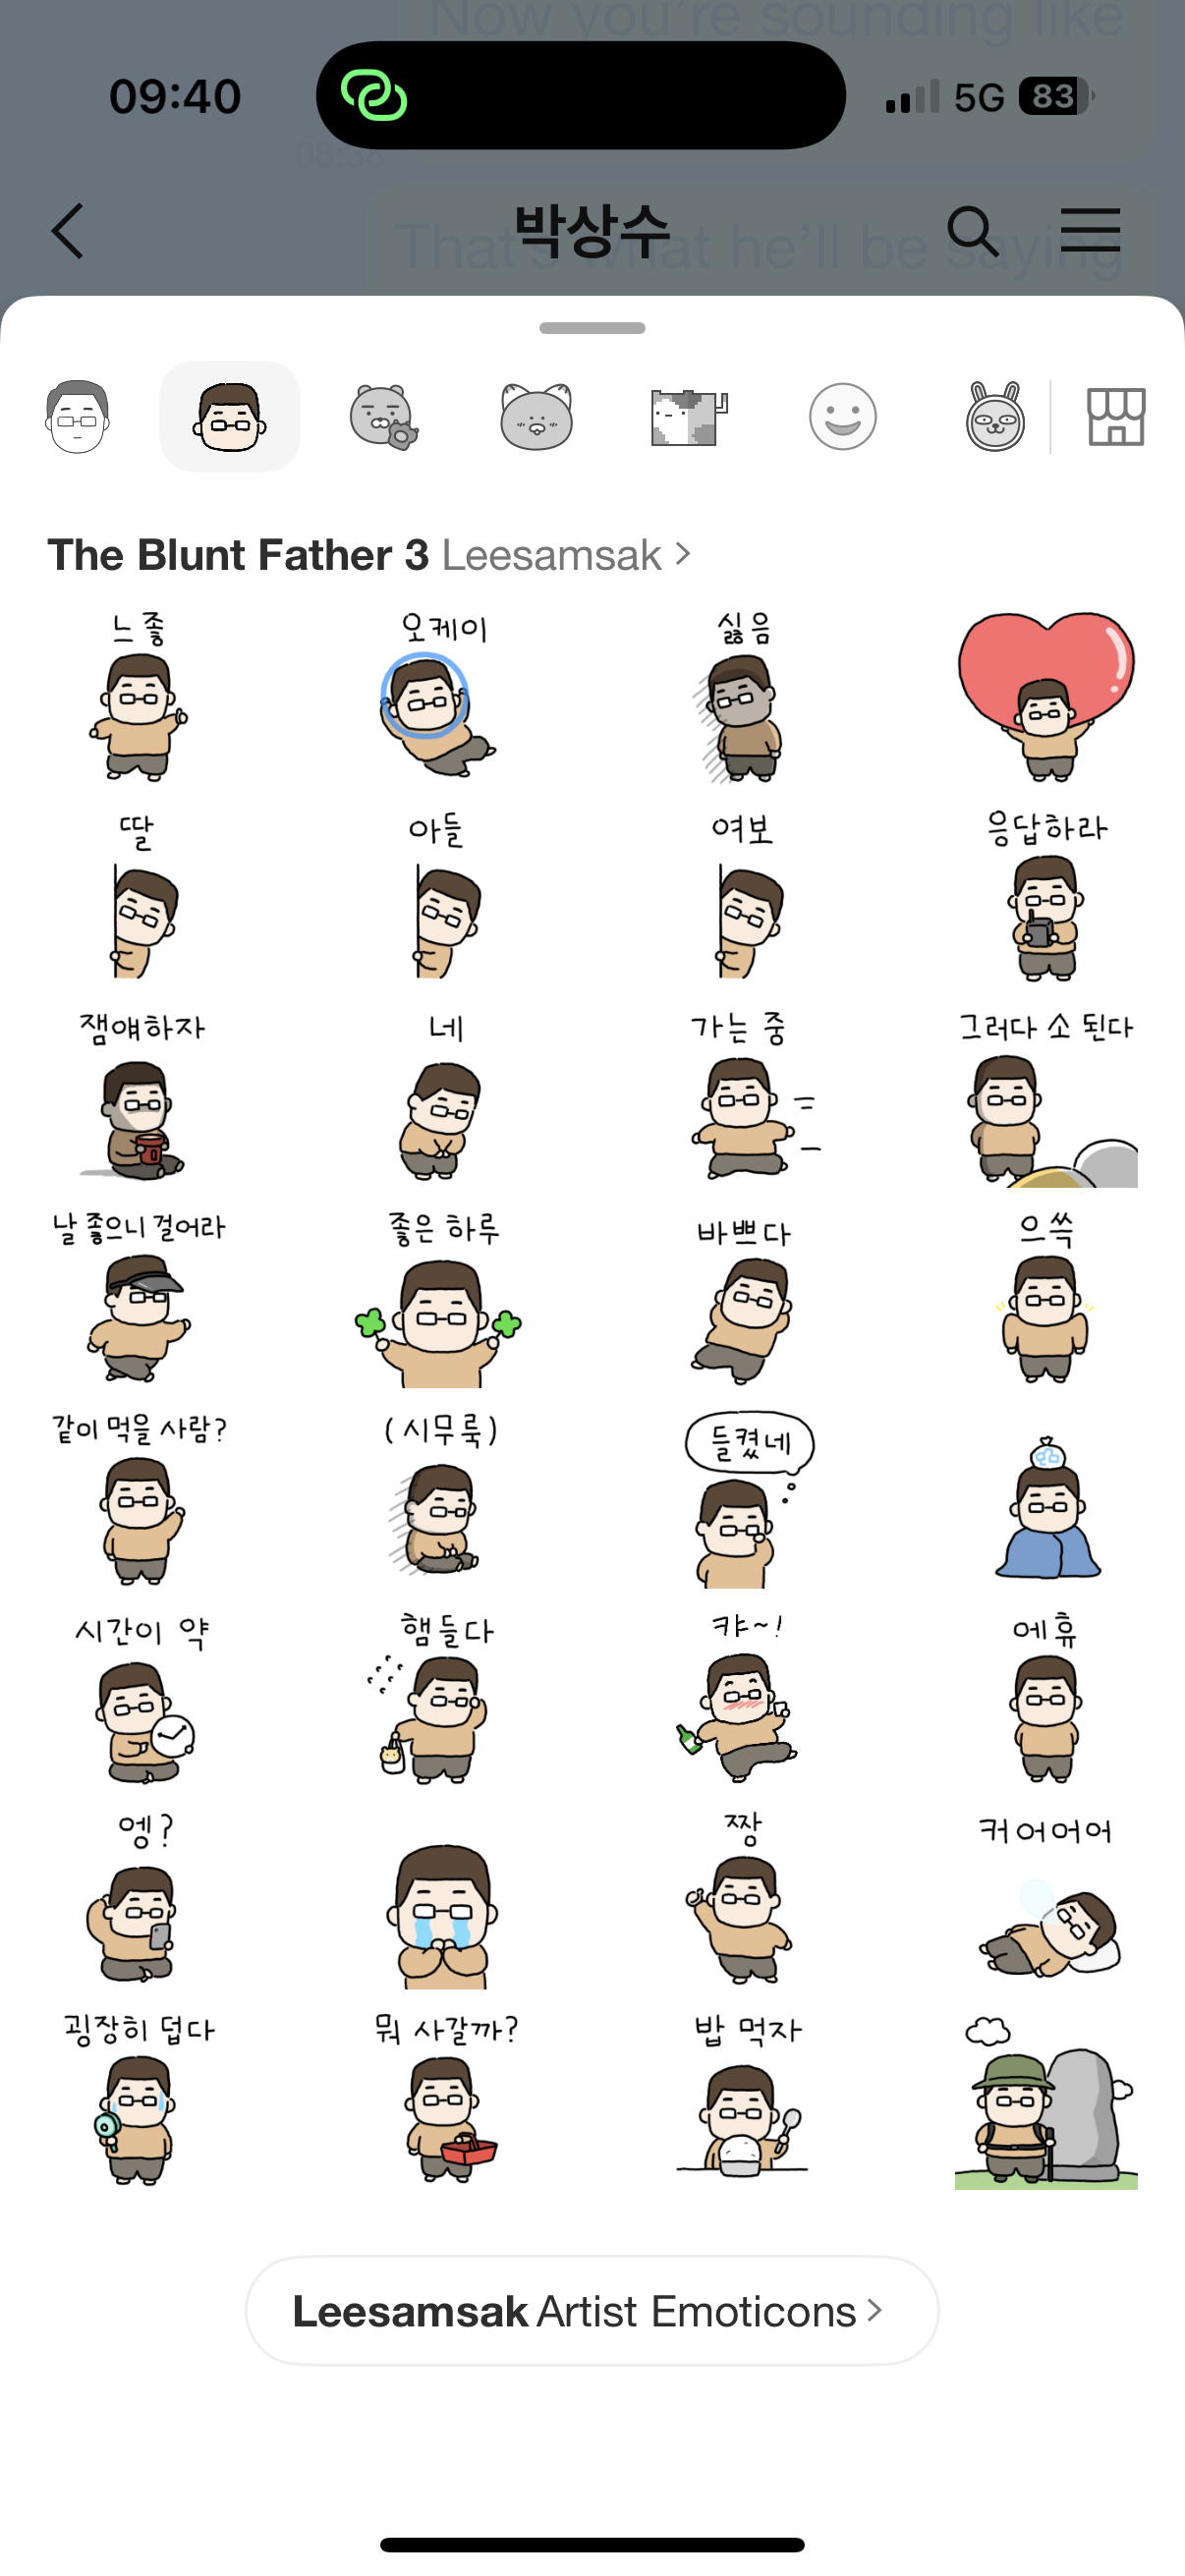
\includegraphics[width=1.04167in,height=\textheight,keepaspectratio]{img/bluntfather3.png}

\end{footnotesize}}

\textbf{Animated GIFs and the Early Internet}\\

\url{https://www.youtube.com/embed/2LzyRcLJdlg}




\end{document}
